%Tema para beamer "CCM3" versión 1
%Desarrollo por Erick David Luna Núñez y 
%Fernanda Barajas Hernandez

\documentclass{beamer}

\usepackage[utf8]{inputenc}
\usepackage{xeCJK}
\usepackage{heuristica}
\usepackage[T1]{fontenc}
\usepackage[heuristica,vvarbb,bigdelims]{newtxmath}
\renewcommand*\oldstylenums[1]{\textosf{#1}}
\usepackage[sfdefault,scaled=.85]{FiraSans}
\usepackage{graphicx}
\usepackage[spanish]{babel} 
\usepackage[pages=some]{background}
\usepackage{listings}
\pagenumbering{arabic}



%%Se define el "environment" teorema
\newtheorem{teorema}{Teorema}

%Definir el autor con el estilo definido (el textbf y el uso del color son herramientas del diseño, no necesario borrar)
\title{\textbf{編譯器期末專題}  }

%Nombre del autor
\author{
    \item 李智修 S08351050
    \item 張聯榮 S09350148
    \item 林佑軒 S09350117
} 

%Fecha o evento en que se presentará la plática
\date{報告日期: 2023/05/23} 


%%Tema de beamer "CCM-3"
\usetheme{ccm3}

\begin{document}
{
    \setbeamertemplate{background}{
        
\includegraphics[width=\the\paperwidth,height=\the\paperheight]{images/P3.png}
    }

    %------------------------------------------------------------
    \begin{frame}
        \titlepage %Necesario para generar la portada
    \end{frame}
} %aquí termina el cambio de fondo

%------------------------------------------------------------
\begin{frame}
\tableofcontents %Imprime la tabla de contenido
\end{frame}

%------------------------------------------------------------
\section{使用環境及工具} %%Título de la sección (Opcional)
\subsection{環境}
\begin{frame}
  \frametitle{使用環境}
  \begin{itemize}
    \item 作業系統: Arch Linux %%[\checkmark] muestra una palomita al inicio de la línea
    \item 系統架構: x86\_64
    \item 
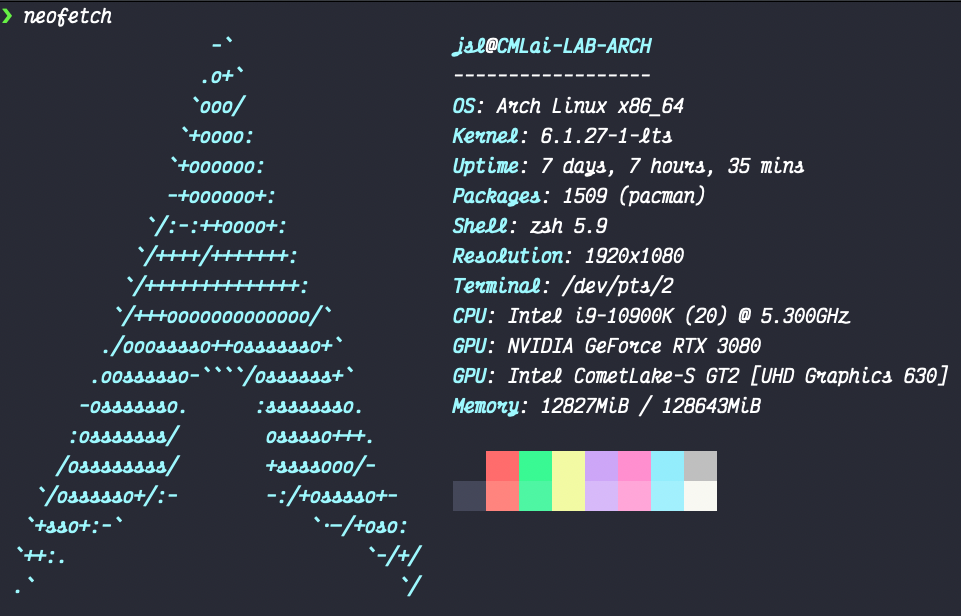
\includegraphics[width=260pt,height=160pt]{images/OS_INFO.png}
  \end{itemize}
\end{frame}

%------------------------------------------------------------
\subsection{工具}
\begin{frame}
  \frametitle{使用工具}
  \begin{itemize}
    \item Makefile: 自動化固定的步驟。
    \item flex, yacc: 將提供的.y, .l檔轉成自制的編譯器。
    \item clang, LLVM: 將程式轉成組合語言,然後編譯成可執行檔。
    \item 
    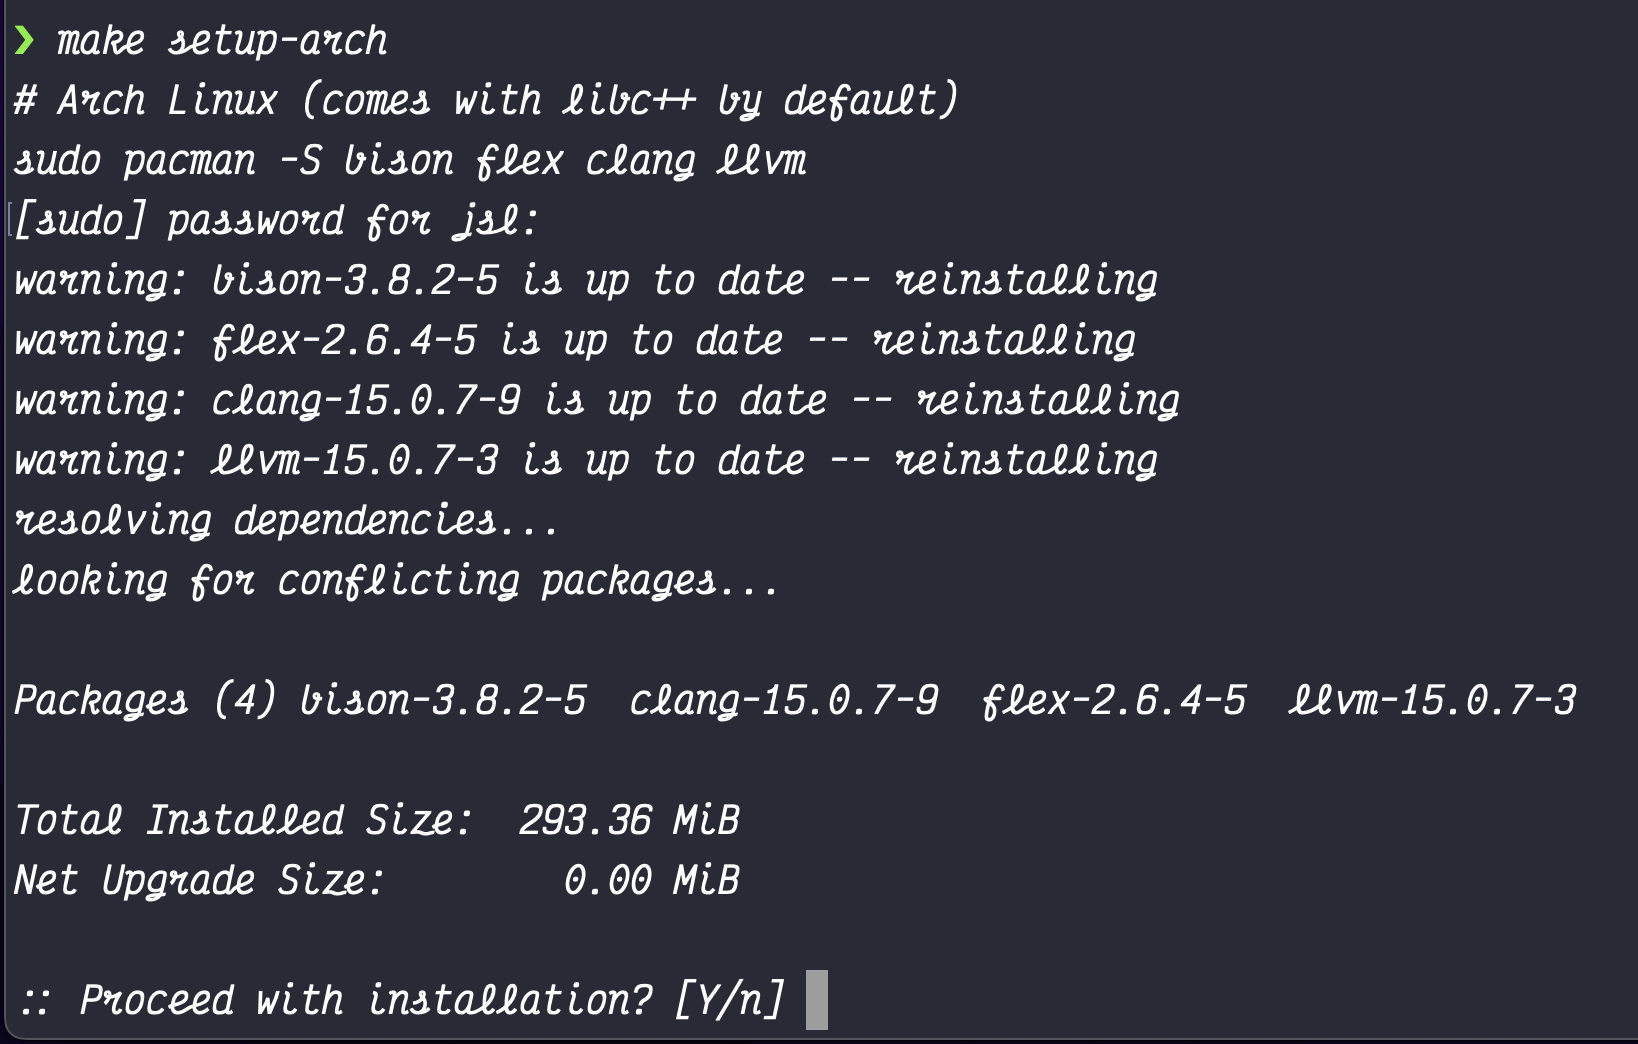
\includegraphics[width=250pt,height=100pt]{238532181-1faf40c2-514c-408a-8031-e7a7a61af23c}
  \end{itemize}
\end{frame}

%------------------------------------------------------------
\section{實作過程}
\subsection{使用flex, yacc生出編譯器}
\begin{frame}{使用flex, yacc生出編譯器}
\begin{itemize}
    \item 我們首先參考了巴哈上的教學\cite{Lex},然後從這兩個地方\cite{ANSILex, ANSIYacc}取得了yacc, lex檔案。
    \item 然而我們發現無法直接使用指令編譯出檔案,因此我們又參考了Github上的討論串\cite{C99Grammars},得知了我們應該使用yacc -d的參數來編譯,而不是直接執行yacc: 
    \item 在同一個討論串中,我們也發現了yacc.y的檔案中需要再增加一個driver的函式(見下頁圖),否則會無法進行編譯。
    \item 其它的都很順例,就照步驟直接做就好了。
\end{itemize}
\end{frame}

%------------------------------------------------------------
\begin{frame}{使用flex, yacc生出編譯器}
\begin{itemize}
    \item 
    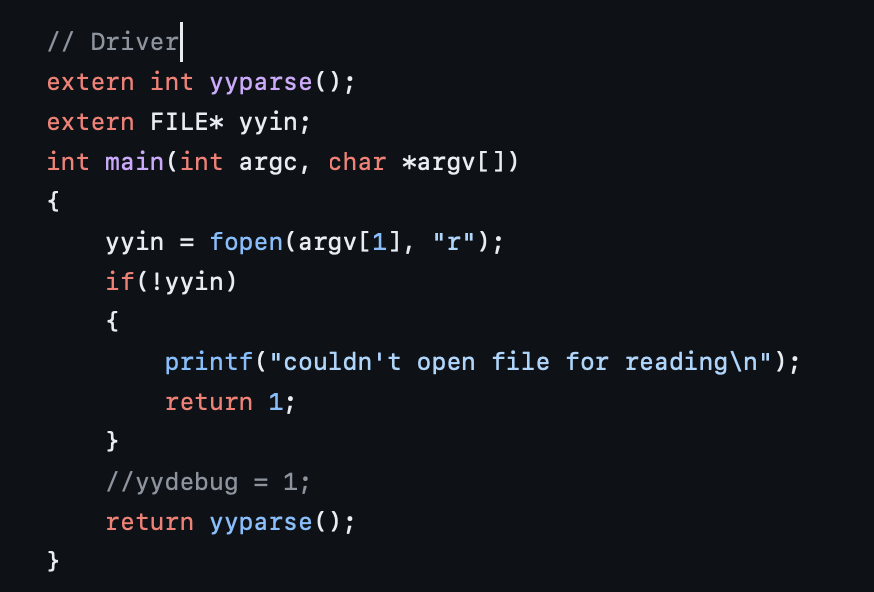
\includegraphics[width=300pt,height=150pt]{截圖 2023-05-16 下午2.36.23}
\end{itemize}
\end{frame}

%------------------------------------------------------------
\begin{frame}{使用flex, yacc生出編譯器}
\begin{itemize}
    \item 執行結果如下:
    \item 
    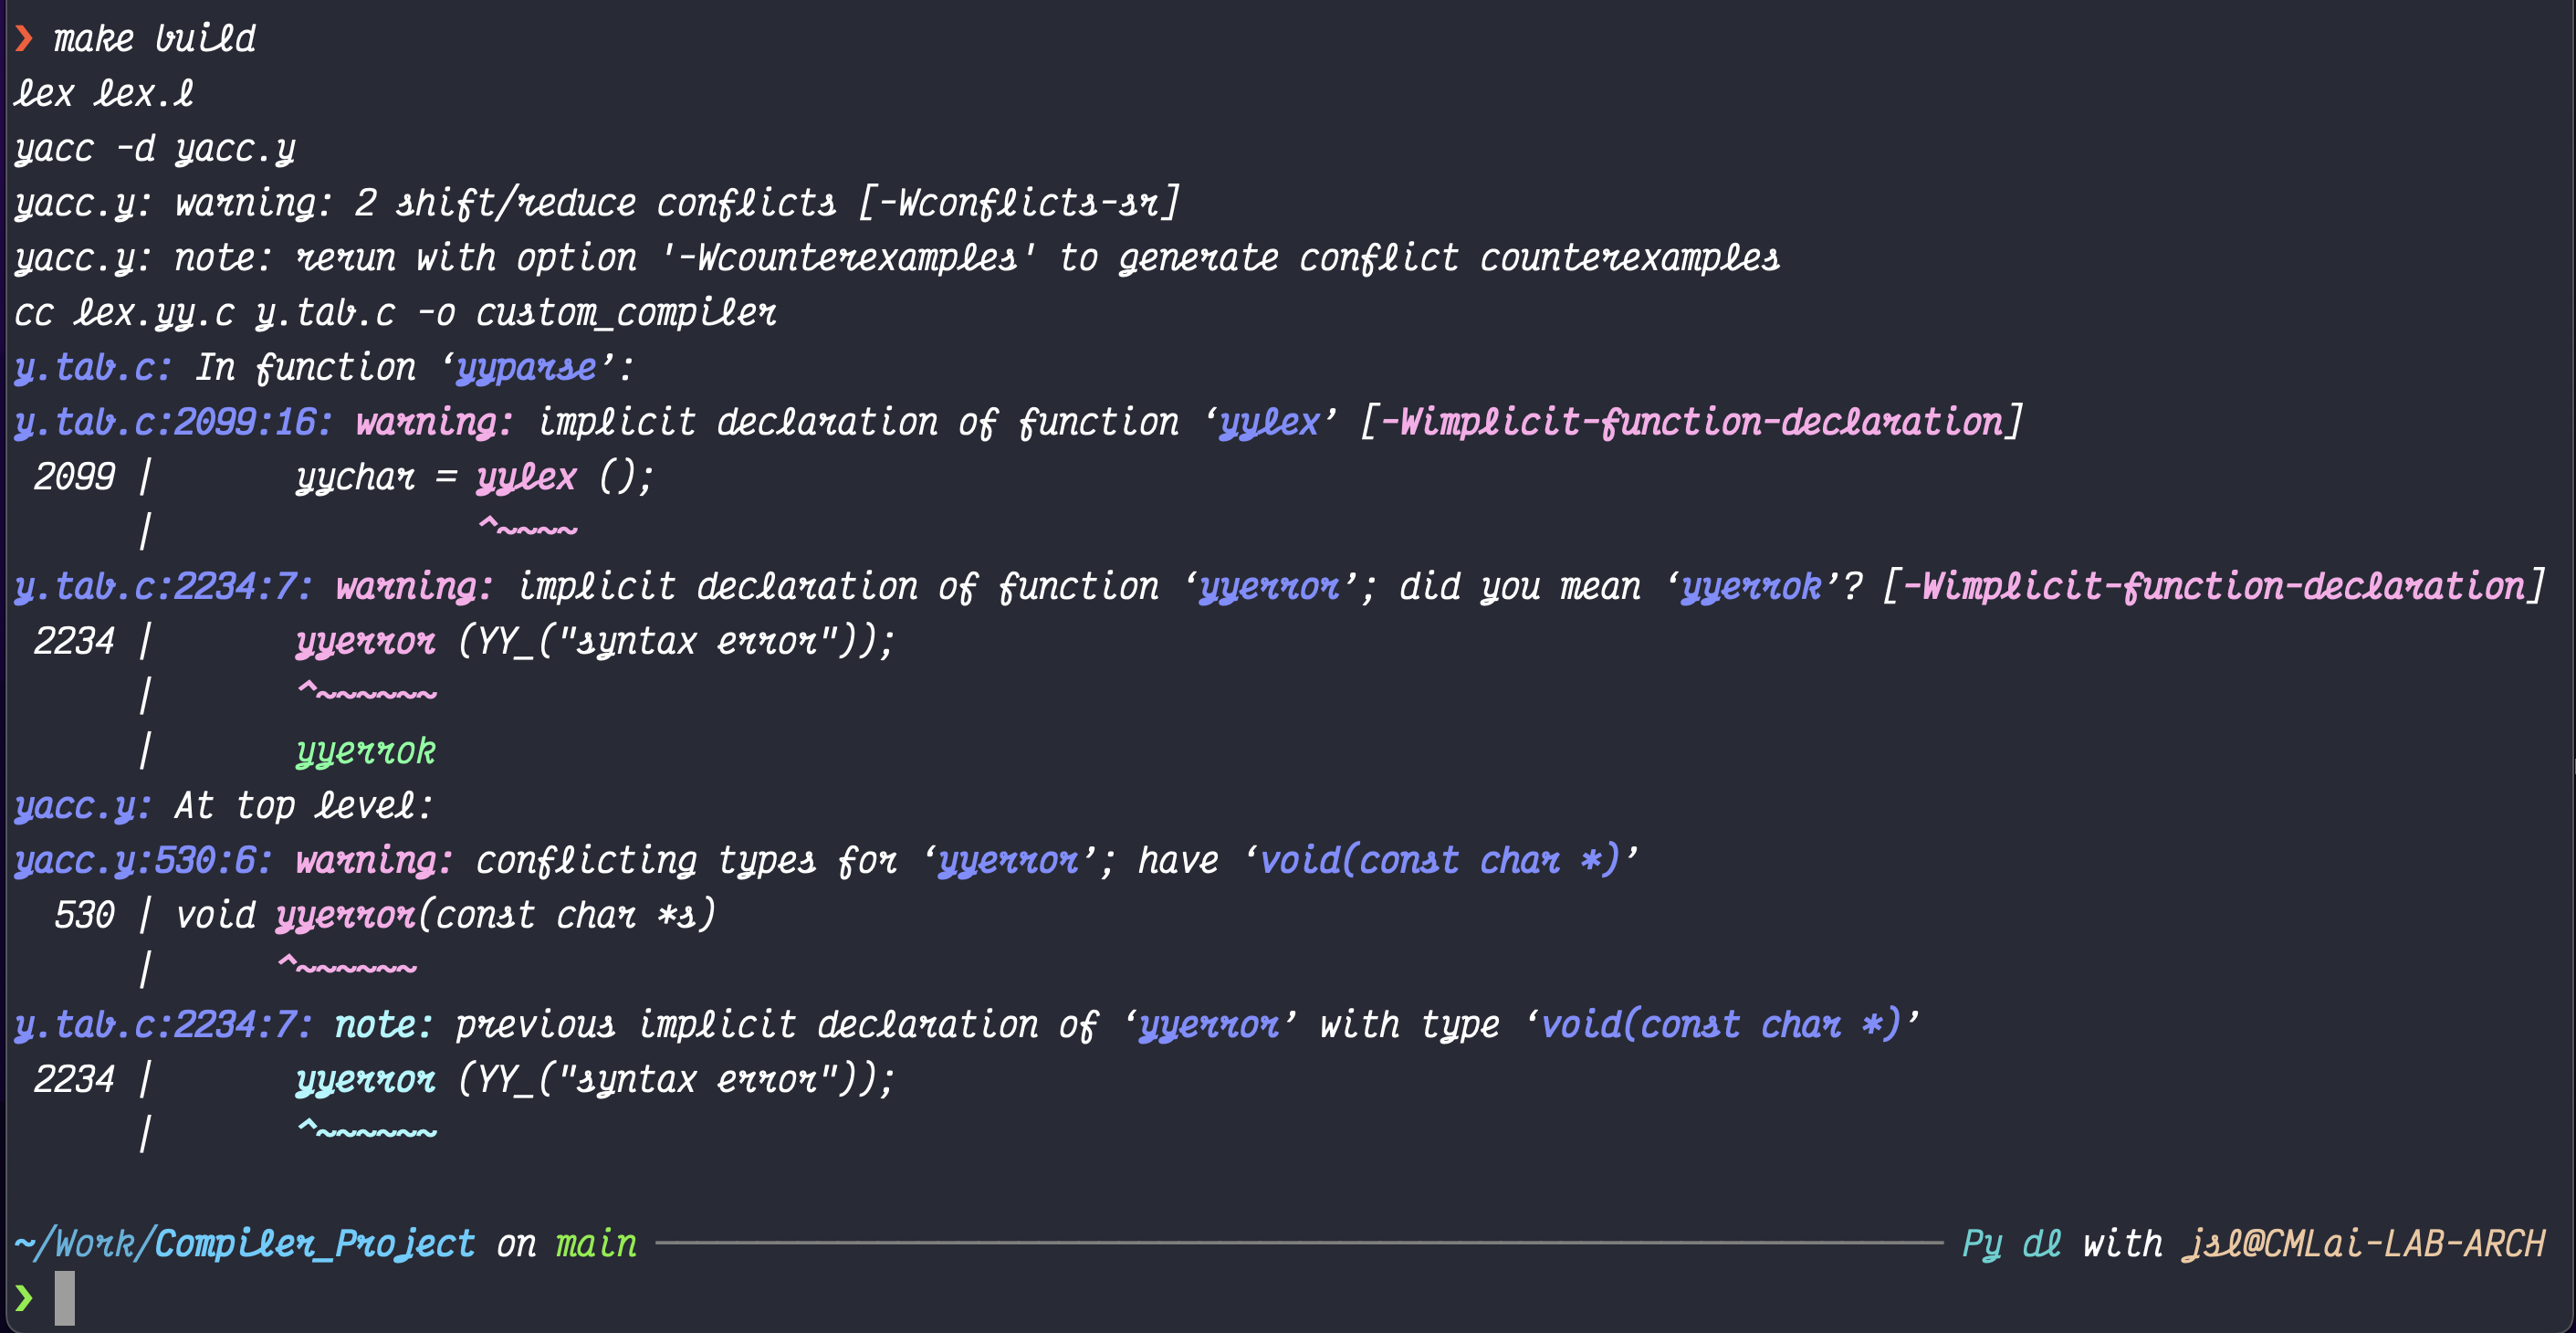
\includegraphics[width=300pt,height=150pt]{238418057-ddf2bca5-cdba-48f9-9b31-7cc684d9087e}
\end{itemize}
\end{frame}
%------------------------------------------------------------
\begin{frame}{使用flex, yacc生出編譯器}
\begin{itemize}
    \item 
    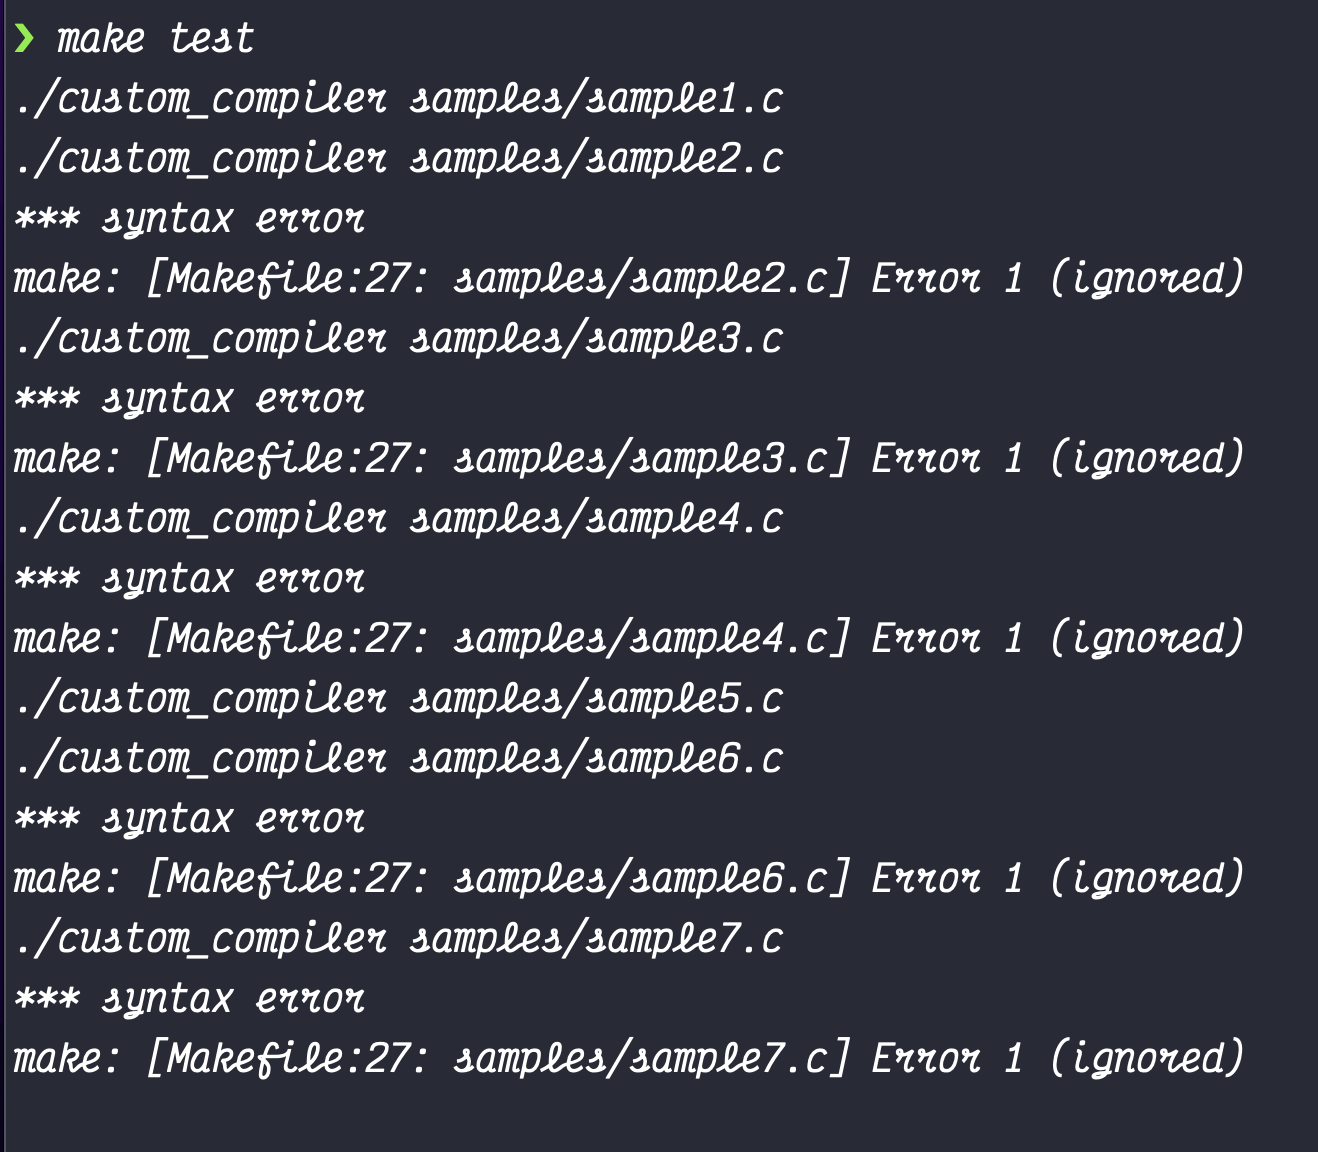
\includegraphics[width=300pt,height=180pt]{238418183-99987aa3-0810-4e34-a41e-92acb99df7cb.png}
\end{itemize}
\end{frame}
%------------------------------------------------------------

\subsection{使用LLVM, clang生出組語、執行檔}
\begin{frame}{使用LLVM, clang生出組語、執行}
\begin{itemize}
    \item 在一開始的時候,我們還不知道如何使用ld指令,就直接加上了上一步生出來的.o檔,所以編譯出來的程式一直顯示Segmentation Fault。
    \item 但是在看了老師提供的教學(pdf)後,發現了其中提到的StackOverflow問題\cite{GccOverflow},讓我們可以跟據上面講的ld進行連接的原理進行我們機器需要的參數調整。
    \item 剩下的都很順利,就按照步驟做就可以了。
    \item 還有一個意外發現,就是ld的參數中,-lc是等價於你直接用/usr/lib/libc.so的效果的。所以我們教學中的指令才不用直接打出libc的路徑,但還是可以使用libc的功能。
\end{itemize}
    
\end{frame}

%------------------------------------------------------------
\begin{frame}{使用LLVM, clang生出組語、執行檔}
\begin{itemize}
    \item 
        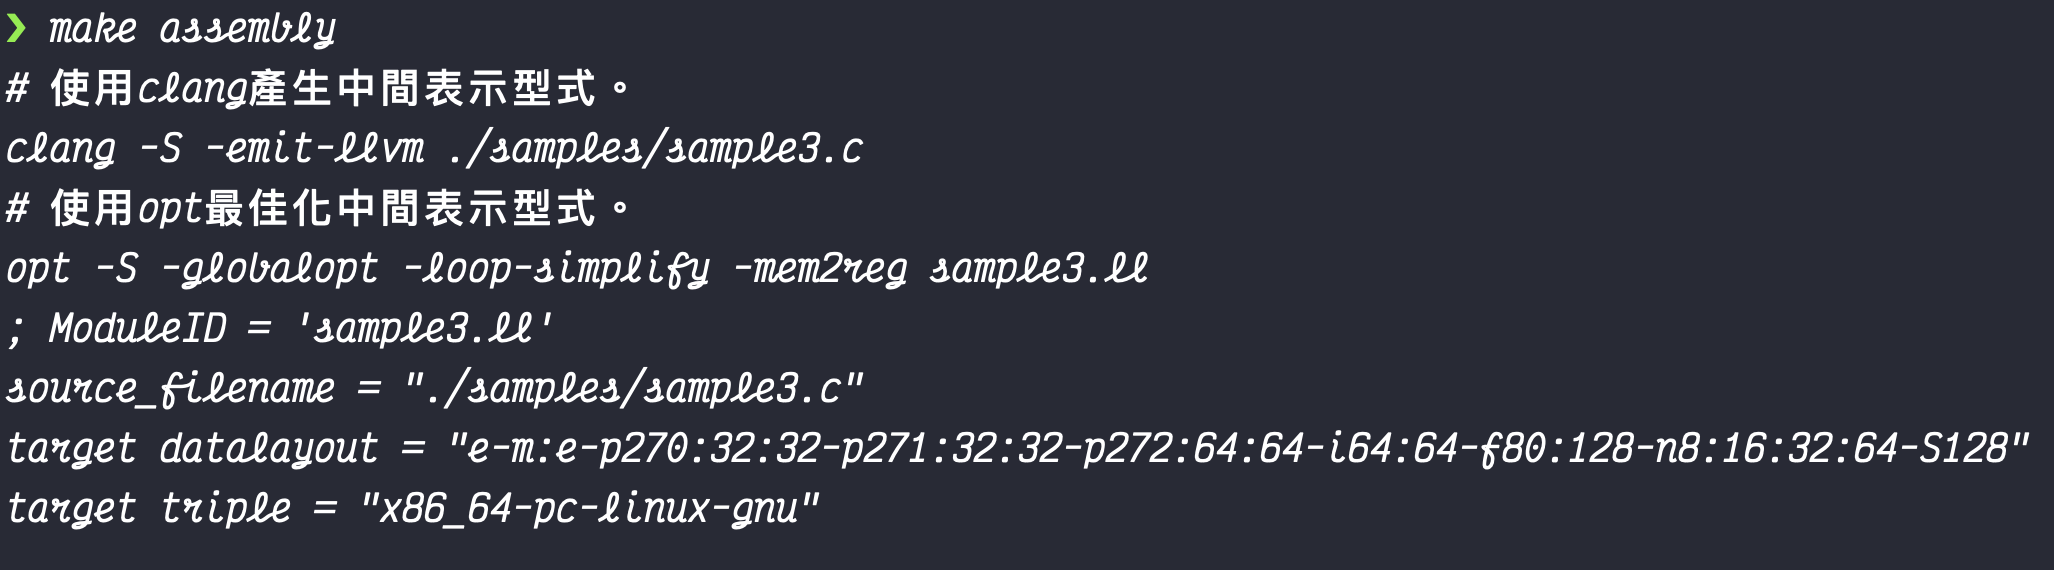
\includegraphics[width=300pt,height=100pt]{238419442-7030003f-ea2c-4296-bcc7-9e7bc5deb41b}
\end{itemize}
\end{frame}

%------------------------------------------------------------
\begin{frame}{使用LLVM, clang生出組語、執行檔}
\begin{itemize}
    
    \item
        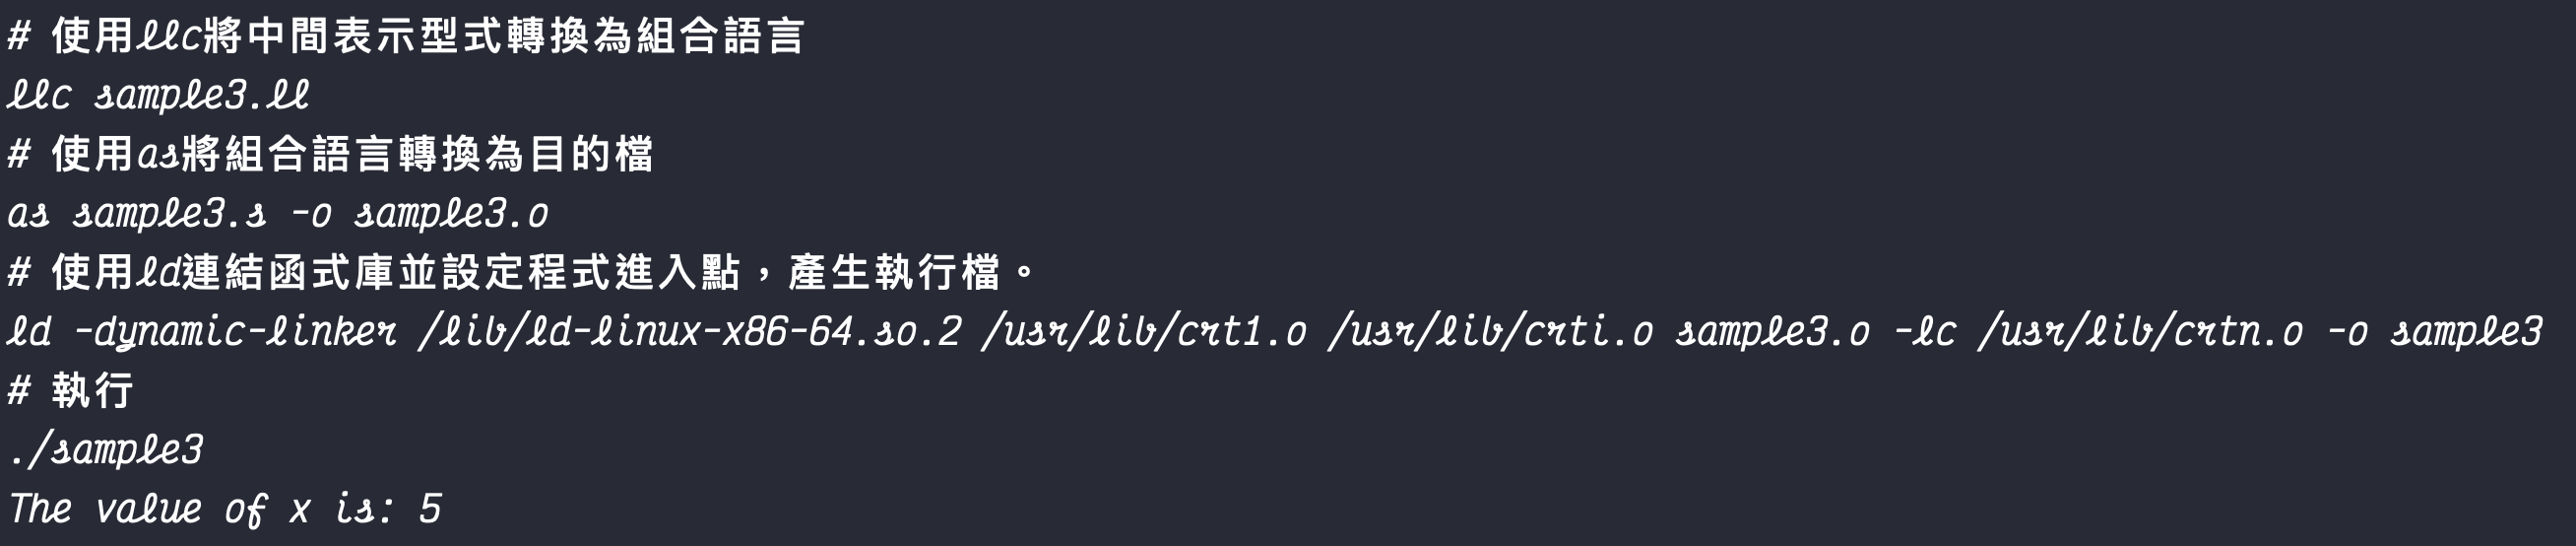
\includegraphics[width=300pt,height=100pt]{238419503-3338260e-882b-48e5-88de-9b67942e9dee}
\end{itemize}
\end{frame}

%------------------------------------------------------------
\section{Makefile實作}
\begin{frame}{使用Makefile加速測試過程}
\begin{itemize}
    \item 大家前面看圖可能有發現,我們的指令都是使用make的指令跑出來的。
    \item 在測試的過程中,通常會需要一個步驟一個步驟debug,因此我們覺得Makefile的簡單跟彈性可能會更合適。
    \item 我們提供了下列指令供測試、設定使用:
    \begin{itemize}
        \item make setup-arch / make setup-ubuntu: 可安裝需要的軟體。
        \item make build: 從.y, .l檔生出我們的編譯器。
        \item make test: 使用samples資料夾下的測試檔案進行我們編譯器的測試。
        \item make assembly: 使用LLVM及其提供的工具生成組合語言、IR、執行檔。
        \item make clean: 清除除了必要之外的中間檔案。
    \end{itemize}
\end{itemize}
\end{frame}

%------------------------------------------------------------
\begin{frame}{Makefile}
\begin{itemize}
    \item 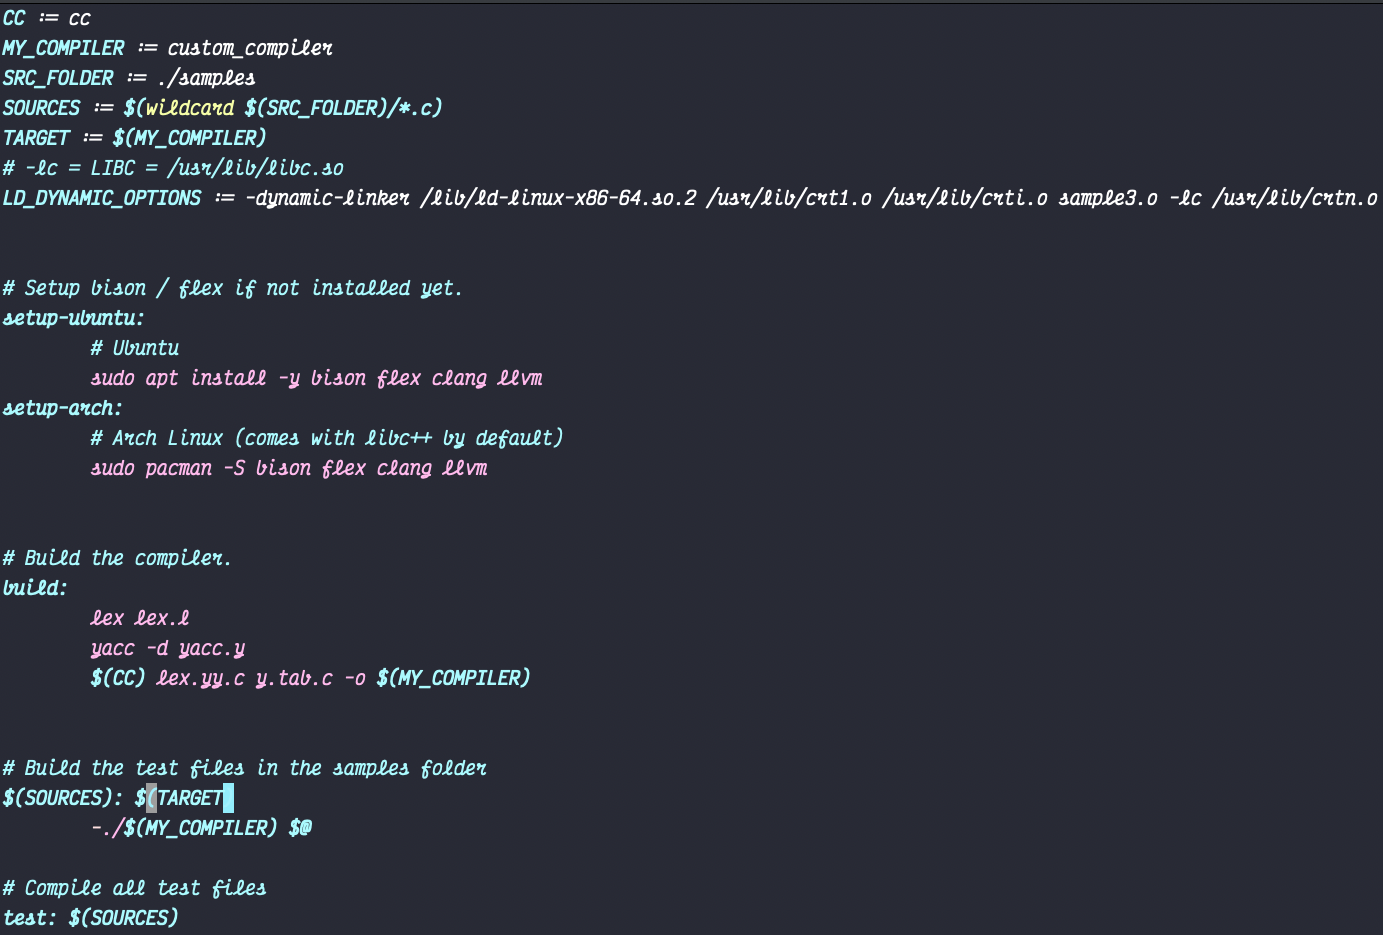
\includegraphics[width=300pt,height=150pt]{makefile1.png}
\end{itemize}
\end{frame}

%------------------------------------------------------------
\begin{frame}{Makefile}
\begin{itemize}
    \item 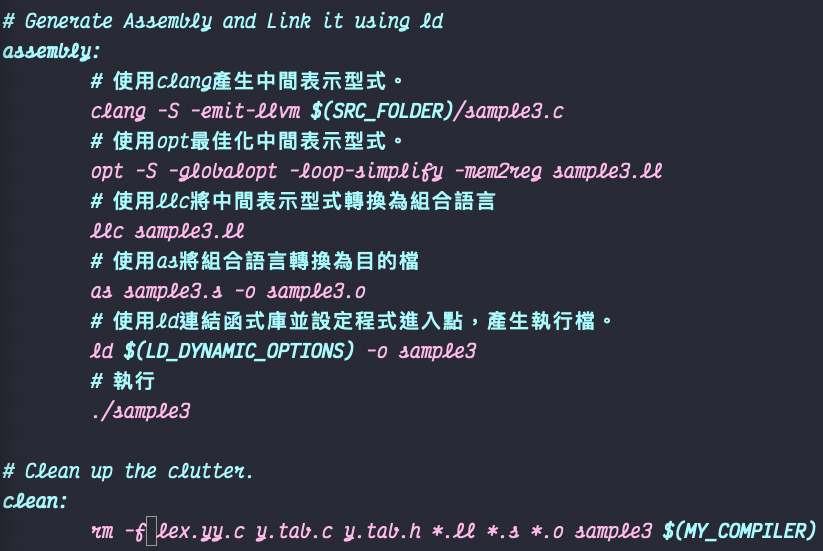
\includegraphics[width=300pt,height=150pt]{makefile2.png}
\end{itemize}
\end{frame}

%------------------------------------------------------------
\section{參考資料}
\begin{frame}{參考資料}
    %posibles estilos para bibliografía: unsrt , siam , plain , ieeetr , alpha , acm , abbrv
    \bibliographystyle{unsrt}
  \bibliography{references}
\end{frame}

%------------------------------------------------------------
\begin{frame}{以上,謝謝大家。}
    
\end{frame}

\end{document}